%%%%%%%%%%%%%%%%%%%%%%%%%%%%%%%%%%%%%%%%%%%%%%%%%%%%%%%%%%%%%%%%%%%%%%%%%%%%%%%%%%%%
% Document data
%%%%%%%%%%%%%%%%%%%%%%%%%%%%%%%%%%%%%%%%%%%%%%%%%%%%%%%%%%%%%%%%%%%%%%%%%%%%%%%%%%%%
\documentclass[12pt]{article} %report allows for chapters
%%%%%%%%%%%%%%%%%%%%%%%%%%%%%%%%%%%%%%%%%%%%%%%%%%%%%%%%%%%%%%%%%%%%%%%%%%%%%%%%%%%%
\usepackage{preamble}
\newcommand{\grad}{\boldsymbol{\vec{\nabla}}}
\newcommand{\curvegamma}{\boldsymbol{\vec{\gamma}}}
\newcommand{\tangentgamma}{\boldsymbol{\dot{\vec{\gamma}}}}
\newcommand{\normalgamma}{\boldsymbol{\ddot{\vec{\gamma}}}}
\newcommand{\vecfieldE}{\boldsymbol{\vec{E}}}
\newcommand{\rhat}{\boldsymbol{\hat{r}}}
\newcommand{\thetahat}{\boldsymbol{\hat{\theta}}}
\newcommand{\phihat}{\boldsymbol{\hat{\phi}}}
\newcommand{\rhohat}{\boldsymbol{\hat{\rho}}}
\newcommand{\unitvec}{\boldsymbol{\hat{n}}}
\newcommand{\vecfieldB}{\boldsymbol{\vec{B}}}
\newcommand{\vecfieldJ}{\boldsymbol{\vec{J}}}
\newcommand{\vecfieldF}{\boldsymbol{\vec{F}}}
\newcommand{\vecfieldV}{\boldsymbol{\vec{V}}}
\newcommand{\vecfieldU}{\boldsymbol{\vec{U}}}

\begin{document}

\begin{center}
   \textsc{\large MATH 272, Homework 3. \emph{Solutions}.}\\
\end{center}
\vspace{.5cm}


\begin{problem}
Show that for any smooth (more than twice differentiable) fields $f(x,y,z)$ and $\vecfieldV(x,y,z)$ that
\begin{enumerate}[(a)]
	\item $\grad \times \left(\grad f\right)=\boldsymbol{\vec{0}}$;
	\item $\grad \cdot \left(\grad \times \vecfieldV\right)=0$.
\end{enumerate}
\end{problem}
\begin{solution}~
    \begin{enumerate}[(a)]
        \item We have that 
        \[
        \grad f = \begin{pmatrix} \frac{\partial f}{\partial x} \\ \frac{\partial f}{\partial y} \\ \frac{\partial f}{\partial z}\end{pmatrix} = \begin{pmatrix} V_1 \\ V_2 \\ V_3 \end{pmatrix}.
        \]
        Taking the curl yields
        \[
        \grad \times \left(\grad f\right) = \begin{pmatrix} \frac{\partial V_3}{\partial y} - \frac{\partial V_2}{\partial z} \\ \frac{\partial V_1}{\partial z} - \frac{\partial V_3}{\partial x} \\ \frac{\partial V_2}{\partial x} - \frac{\partial V_1}{\partial y} \end{pmatrix} = 
        \begin{pmatrix} \frac{\partial^2 f}{\partial z\partial y} - \frac{\partial^2 f}{\partial y\partial z} \\ \frac{\partial^2 f}{\partial x\partial z} - \frac{\partial^2 f}{\partial z \partial x} \\ \frac{\partial^2 f}{\partial y\partial x} - \frac{\partial f}{\partial x\partial y} \end{pmatrix}= \begin{pmatrix} 0 \\ 0 \\ 0 \end{pmatrix},
        \]
        since partial derivatives commute for any smooth scalar field.
        
        \item First, the curl is
        \[
        \grad \times \vecfieldV = \begin{pmatrix} \frac{\partial V_3}{\partial y} - \frac{\partial V_2}{\partial z} \\ \frac{\partial V_1}{\partial z} - \frac{\partial V_3}{\partial x} \\ \frac{\partial V_2}{\partial x} - \frac{\partial V_1}{\partial y} \end{pmatrix},
        \]
        and we can take the divergence
        \begin{align*}
            \grad \cdot \left(\grad \times \vecfieldV\right) &= \frac{\partial}{\partial x} \left(\frac{\partial V_3}{\partial y} - \frac{\partial V_2}{\partial z}\right) +  \frac{\partial}{\partial y} \left(\frac{\partial V_1}{\partial z} - \frac{\partial V_3}{\partial x}\right) +  \frac{\partial}{\partial z} \left(\frac{\partial V_2}{\partial x} - \frac{\partial V_1}{\partial y}\right)\\
            &= 0,
        \end{align*}
        again since partial derivatives commute.
    \end{enumerate}
\end{solution}

\newpage
\begin{problem}
	Let 
	\[
	\vecfieldU(x,y,z) = \begin{pmatrix} -y \\ x \\ 0 \end{pmatrix} \qquad \textrm{and} \qquad \vecfieldV(x,y,z) = \begin{pmatrix} 2x \\ 2y \\ 2z \end{pmatrix},
	\] 
	be vector fields.  
	\begin{enumerate}[(a)]
		\item Explain why there exists no potential function $\phi(x,y,z)$ for the vector field $\vecfieldU$.
		\item Explain why there does exist a potential function $\phi(x,y,z)$ for the field $\vecfieldV$.
		\item Compute the potential function for $\vecfieldV$.
	\end{enumerate}
\end{problem}
\begin{solution}~
    \begin{enumerate}[(a)]
        \item There exists a potential function if the curl of $\vecfieldU$ is zero.  So, taking the curl we find
        \[
        \grad \times \vecfieldU = \begin{pmatrix} 0 \\ 0 \\ 2 \end{pmatrix},
        \]
        which is nonzero. Thus, there cannot be a potential function for $\vecfieldU$.
        
        \item Likewise, taking the curl for $\vecfieldV$ we get
        \[
            \grad\times \vecfieldU = \begin{pmatrix} 0 \\ 0 \\ 0 \end{pmatrix}.
        \]
        Hence, there must be a potential function for $\vecfieldV$.  
        
        \item To compute the potential $\phi(x,y,z)$, we integrate $V_1$ with respect to $x$, $V_2$ with respect to $y$, and $V_3$ with respect to $z$.  This yields
        \begin{align*}
            \phi(x,y,z) &= \int 2x dx = x^2+\psi_1(y,z)\\
            \phi(x,y,z) &= \int 2y dy = y^2+\psi_2(x,z)\\
            \phi(x,y,z) &= \int 2z dz = z^2+\psi_3(x,y).
        \end{align*}
        Since these are all equal, we must have that
        \[
        \boxed{\phi(x,y,z) = x^2+y^2+z^2+C,}
        \]
        where $C$ is a constant.
    \end{enumerate}
\end{solution}

\newpage
\begin{problem}
Consider the two dimensional scalar field $T(x,y)=x+y$ that describes the temperature on the square plate $\Omega$ given by the set $0\leq x,y \leq 1$.  Compare the two answers you get!
\begin{enumerate}[(a)]
	\item Compute the integral
	\[
	\int_\Omega T d\Omega.
	\]
	\item Let $\curvegamma$ be the curve that traverses the boundary of the square plate in the counterclockwise direction.  Compute
	\[
	\int_{\curvegamma} T d\curvegamma. 
	\]
\end{enumerate}
\end{problem}
\begin{solution} ~
	\begin{enumerate}[(a)]
		\item We take
		\begin{align*}
			\iint_\Omega T(x,y)d\Omega &= \int_0^1 \int_0^1 x+y dxdy\\
			&= \int_0^1 \left.\left(\frac{1}{2}x^2+xy\right)\right\vert_0^1 dy\\
			&= \int_0^1 \frac{1}{2} + y dy\\
			&= \left.\left(\frac{1}{2}y + \frac{1}{2}y^2\right)\right\vert_0^1\\
			&= 1.
		\end{align*}
		\item	First, note that there are four straight curves that parameterize the boundary of the plate.  Namely, we can choose the parameterizations 
		\[
		\curvegamma_1(t) = \begin{pmatrix} t \\ 0 \end{pmatrix} \quad \curvegamma_2(t) = \begin{pmatrix} 1 \\ t \end{pmatrix} \quad \curvegamma_1(t) = \begin{pmatrix} 1-t \\ 1 \end{pmatrix} \quad \curvegamma_1(t) = \begin{pmatrix} 0 \\ 1-t \end{pmatrix},
		\]
		Note that there are many other parameterizations that work. We can see the chosen curves in this figure:
		\begin{figure}[H]
			\centering
			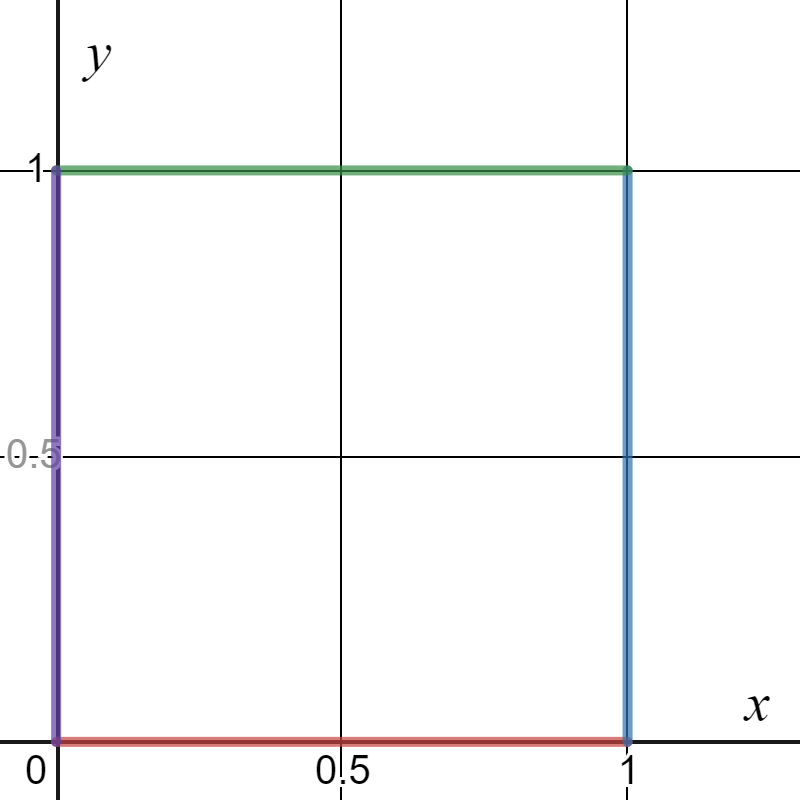
\includegraphics[width=.6\textwidth]{figures/plate_boundary.png}
		\end{figure}
		Thus, our integral can be written as
		\[
		\int_{\curvegamma} T(\curvegamma) d\curvegamma = \int_{\curvegamma_1} T(\curvegamma) d\curvegamma_1 + \int_{\curvegamma_2} T(\curvegamma) d\curvegamma_2 + \int_{\curvegamma_3} T(\curvegamma) d\curvegamma_3 + \int_{\curvegamma_4} T(\curvegamma) d\curvegamma_4.
		\]
		Then, we can compute each integral on the right hand side.
		\begin{align*}
			\int_{\curvegamma_1} T(\curvegamma_1) d\curvegamma_1 &= \int_0^1 T(\curvegamma_1(t))\left|\tangentgamma_1(t)\right|dt\\
			&= \int_0^1 T(t,0) dt\\
			&= \int_0^1 t dt\\
			&= 1.
		\end{align*}
		Similarly, 
		\begin{align*}
				\int_{\curvegamma_2} T(\curvegamma_2) d\curvegamma_2 &= \int_0^1 T(\curvegamma_2(t))\left|\tangentgamma_2(t)\right|dt\\
				&= \int_0^1 T(1,t) dt\\
				&= \int_0^1 1+t dt\\
				&= \left.\left(t+\frac{1}{2}t^2\right)\right\vert_0^1\\
				&= \frac{3}{2}.
		\end{align*}	
		Again,
		\begin{align*}
				\int_{\curvegamma_3} T(\curvegamma_3) d\curvegamma_3 &= \int_0^1 T(\curvegamma_3(t))\left|\tangentgamma_3(t)\right|dt\\
				&= \int_0^1 T(1-t,1) dt\\
				&= \int_0^1 (1-t)+1 dt\\
				&= \int_0^1 2-tdt\\
				&= \left.\left( 2t-\frac{1}{2}t^2\right)\right\vert_0^1\\
				&= \frac{3}{2}.
		\end{align*}			
		Lastly,
		\begin{align*}
			\int_{\curvegamma_4} T(\curvegamma_4) d\curvegamma_4 &= \int_0^1 T(\curvegamma_4(t))\left|\tangentgamma_4(t)\right|dt\\
			&= \int_0^1 T(0,1-t) dt\\
			&= \int_0^1 1-t dt\\
			&= \left.\left(t-\frac{1}{2}t^2\right)\right\vert_0^1\\
			&= \frac{1}{2}.
		\end{align*}	
	\end{enumerate}
	Thus, we have
	\[
	\boxed{\int_{\curvegamma} T(\curvegamma) d\curvegamma = 1+\frac{3}{2}+\frac{3}{2}+\frac{1}{2} = \frac{9}{2}.}
	\]
\end{solution}

\newpage
\begin{problem}
Let $f(x,y,z)=2xy+e^{xz}+\sin(y)$ be a scalar field. Integrate $f$ over the triangular prism $\Omega$ defined by taking the half triangle of the unit square in the $xy$-plane satisfying $x\leq y$ and with height 4 above the $xy$-plane.
\end{problem}
\begin{solution}
We wish to compute a triple integral
\[
\iiint_{\Omega} f d\Omega = \int_{z=?}^{z=?} \int_{y=?}^{y=?} \int_{x=?}^{x=?} 2xy +e^{xz} + \sin(y) dxdydz.
\]
The challenge is predominantly in determining the bounds of integration based on the geometry of $\Omega$. 

Based off the wording of the problem, let us begin with the unit square in the $xy$-plane which is the set of points $x\in [0,1]$ and $y\in [0,1]$. We can realize this in the following figure.
\begin{figure}[H]
    \centering
    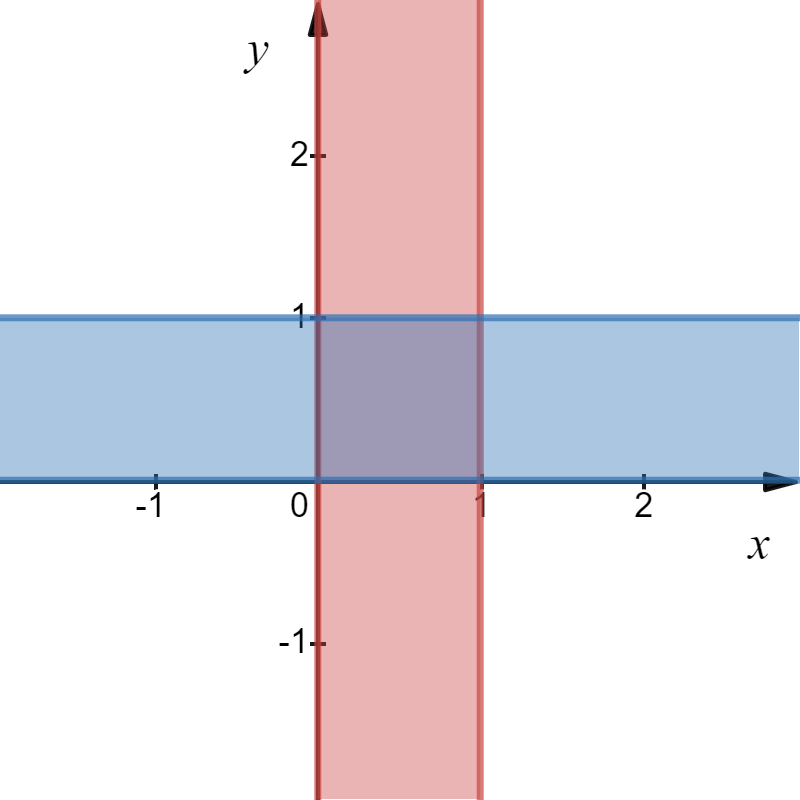
\includegraphics[width=.6\textwidth]{figures/bounds_1.png}
    \caption{Red band is the set of points $x\in [0,1]$ and the blue band is the set of points $y\in [0,1]$. Where they overlap is the unit square.}
\end{figure}
Yet, we want to create a half triangle of this square subject to the constraint $x\leq y$. Thus, we get the following figure.
\begin{figure}[H]
    \centering
    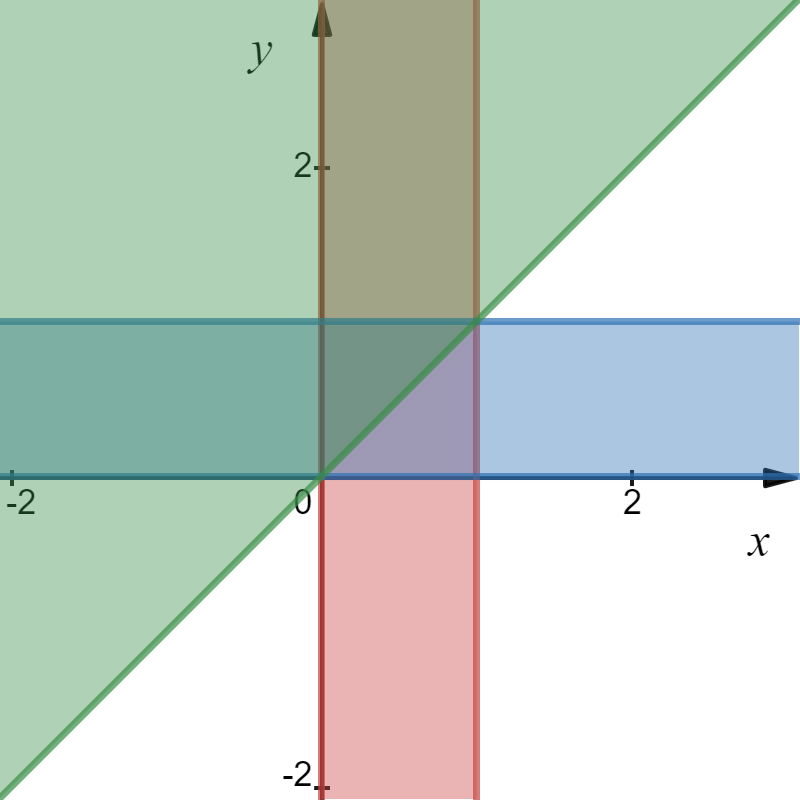
\includegraphics[width=.6\textwidth]{figures/bounds_2.png}
    \caption{Additional green area is the constraint $x\leq y$.}
\end{figure}
Where every color overlaps is the domain in the $xy$-plane we wish to integrate over. Following the figure and given constraint for intuition, we realize that the bounds for $x$ must depend on $y$. Note, the bounds for $y$ \emph{cannot} depend on $x$ if we integrate $y$ \emph{after} $x$! We can see that the bounds $0\leq x \leq y$ yield the following figure.
\begin{figure}[H]
    \centering
    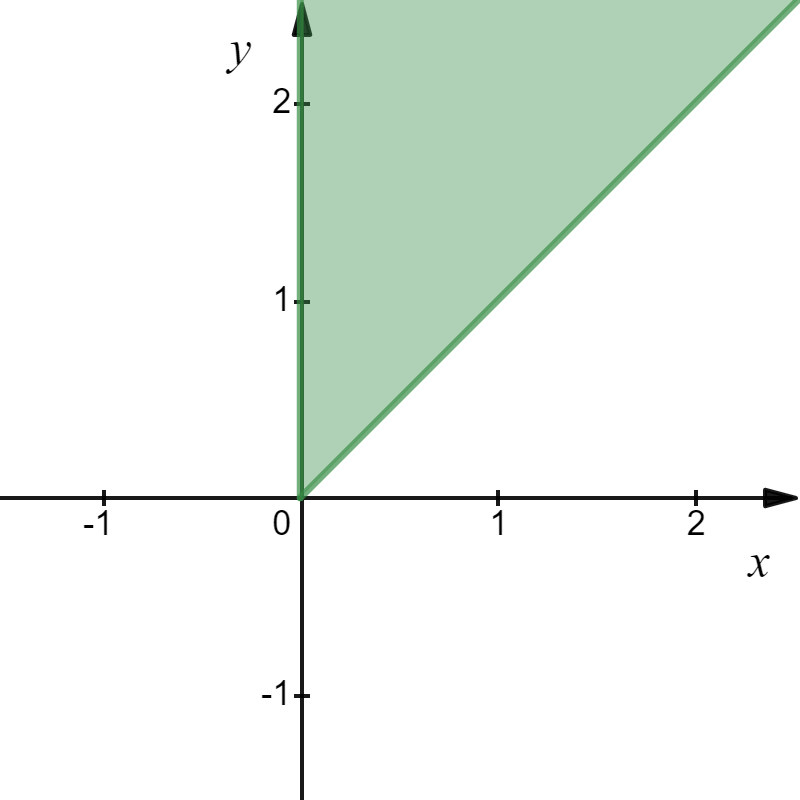
\includegraphics[width=.6\textwidth]{figures/bounds_3.png}
    \caption{The region where $0\leq x\leq y$.}
\end{figure}
Now, we have determined bounds for $x$ via this analysis and we still need to determine bounds for both $y$ and $z$ (which we have not discussed at all yet!). The bounds for $y$ can be seen by investigating the previous figures. We need $0\leq y \leq 1$ in order to integrate over the half triangle of the unit square -- no more, no less. Hence, we now can put
\[
\iiint_{\Omega} f d\Omega = \int_{z=?}^{z=?} \int_{y=0}^{y=1} \int_{x=0}^{x=y} 2xy +e^{xz} + \sin(y) dxdydz.
\]
Finally, the triangular prism is built by extending this triangle out of the plane in the $z$-direction. Specifically, the prism should go up a height of 4 above the $xy$-plane, and so $z \in [0,4]$. Thus, we now have an integral to compute
\begin{align*}
\iiint_{\Omega} f d\Omega &= \int_{z=0}^{z=4} \int_{y=0}^{y=1} \int_{x=0}^{x=y} 2xy +e^{xz} + \sin(y) dxdydz\\
&\approx 7.4725.
\end{align*}
This integral was computed using WolframAlpha by inputting:
\begin{verbatim}
integrate[integrate[integrate[2xy+e^(xz)+sin(y),{x,0,y}],{y,0,1}],{z,0,4}]
\end{verbatim}
\end{solution}

\newpage
\begin{problem}
Consider $f(x,y)= 3x^4+x^3-18x^2y^2-3xy^2+3y^4$. 
\begin{enumerate}[(a)]
    \item Show $\Delta f = 0$.
    \item Find the surface normal to the graph of $f$.
\end{enumerate}
\end{problem}
\begin{solution}~
\begin{enumerate}[(a)]
    \item We have
    \[
    \frac{\partial^2 f}{\partial x^2} = 6(6x^2+x-6y^2),
    \]
    which was computed using WolframAlpha by inputting:
    \begin{verbatim}
    D[3x^4+x^3-18x^2y^2-3xy^2+3y^4, {x,2}]
    \end{verbatim}
    Likewise,
    \[
    \frac{\partial^2 f}{\partial y^2} = -6(6x^2+x-6y^2),
    \]
    which again was computed via WolframAlpha by:
    \begin{verbatim}
    D[3x^4+x^3-18x^2y^2-3xy^2+3y^4, {y,2}]
    \end{verbatim}
    Thus,
    \[
    \Delta f = \frac{\partial^2 f}{\partial x^2} + \frac{\partial^2 f}{\partial y^2} = 0.
    \]
    \emph{Note: you can actually create a polynomial $f$ satisfying $\Delta f = 0$ (i.e., it is harmonic) by taking the real or imaginary part of any complex polynomial in the variable $z=x+iy$. This is how I created this!}

    \item We have the equation to the normal of a graph of $f(x,y)$ given by
    \[
        \unitvec = \frac{1}{\sqrt{1+\left(\frac{\partial f}{\partial x}\right)^2 + \left(\frac{\partial f}{\partial y}\right)^2}} \begin{pmatrix} -\frac{\partial f}{\partial x} \\ -\frac{\partial f}{\partial y} \\ 1 \end{pmatrix}.
    \]
    We have
    \[
    \frac{\partial f}{\partial x} = 3(4x^3+x^2-12xy^2-y^2) \qquad \textrm{and} \qquad \frac{\partial f}{\partial y} = -6y(6x^2+x-2y^2).
    \]
    Thus
    \[
    \boxed{\unitvec = \frac{1}{\sqrt{1 + \left( 3(4x^3+x^2-12xy^2-y^2) \right)^2 + \left( -6y(6x^2+x-2y^2) \right)^2 }} \begin{pmatrix} -3(4x^3+x^2-12xy^2-y^2) \\ 6y(6x^2+x-2y^2) \\ 1 \end{pmatrix}.}
    \]
    No real need to simplify further unless we are asked to.
\end{enumerate}
\end{solution}

\newpage
\begin{problem} 
Parameterize the following either implicitly or explicitly. In Cartesian coordinates, find the parameterization of the normal vector as well.
\begin{enumerate}[(a)]
	\item The plane perpendicular to the vector $\vecv = \xhat + \yhat + \zhat$ passing through the point $(1,1,1)$.
	\item The upper half of the unit disk in the $xy$-plane.
	\item The surface of the unit sphere in $\R^3$.
\end{enumerate}
\end{problem}
\begin{solution}~
\begin{enumerate}[(a)]
    \item The equation for a plane passing through a point $(x_0,y_0,z_0)$ perpendicular to a vector $\begin{pmatrix} a \\ b \\ c \end{pmatrix}$ is given by the implicit equation
    \[
    a(x-x_0)+b(y-y_0) + c(z-z_0) = 0.
    \]
    We are given the vector $\vecv = \begin{pmatrix} 1 \\ 1 \\ 1 \end{pmatrix}$ and $x_0=1$, $y_0=1$, and $z_0=1$ so we arrive at
    \[ 
    (x-1)+(y-1)+(z-1)=0.
    \]
    We plot this here.
    \begin{figure}[H]
        \centering
        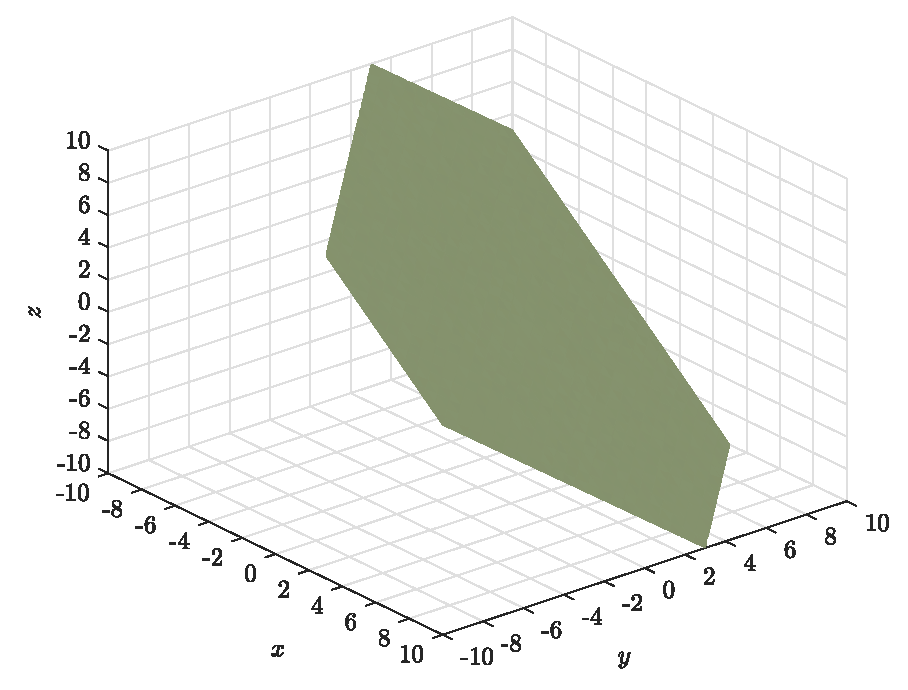
\includegraphics[width=.6\textwidth]{figures/plane}
        \caption{A plot of the plane satisfying our restrictions. Note the plane extends infinitely, but it is cropped by the axes in Matlab.}
    \end{figure}
    The normal vector is constant on a plane and is already being described via $\vecv$. To get the normal vector, we simply normalize $\vecv$ and we find
    \[
    \unitvec = \frac{\vecv}{|\vecv|} = \frac{1}{\sqrt{3}} \begin{pmatrix} 1 \\ 1 \\ 1 \end{pmatrix}.
    \]
    It should be noted that flat surfaces will have constant normals!

    \item Since we are trying to determine a parameterization of the upper half of the unit disk in the $xy$-plane, we may first try to describe bits and pieces of this first. Namely, we have an equation for the unit circle in the $xy$-plane given by the equation
    \[
    x^2+y^2 = 1.
    \]
    Let's think about what this equation is saying a bit. Recall that the distance from the origin $\zerovec$ to the point $(x,y)$ in the $xy$-plane is $\sqrt{x^2+y^2}$ by the Pythagorean theorem. So, this equation is asking for all the points exactly a distance 1 away from the origin. Thus, if we wish to include the interior points, these are just the points that have a distance less than or equal to 1 from the origin. Hence, we should take
    \[
    x^2+y^2\leq 1,
    \]
    which we can graph.
    \begin{figure}[H]
        \centering
        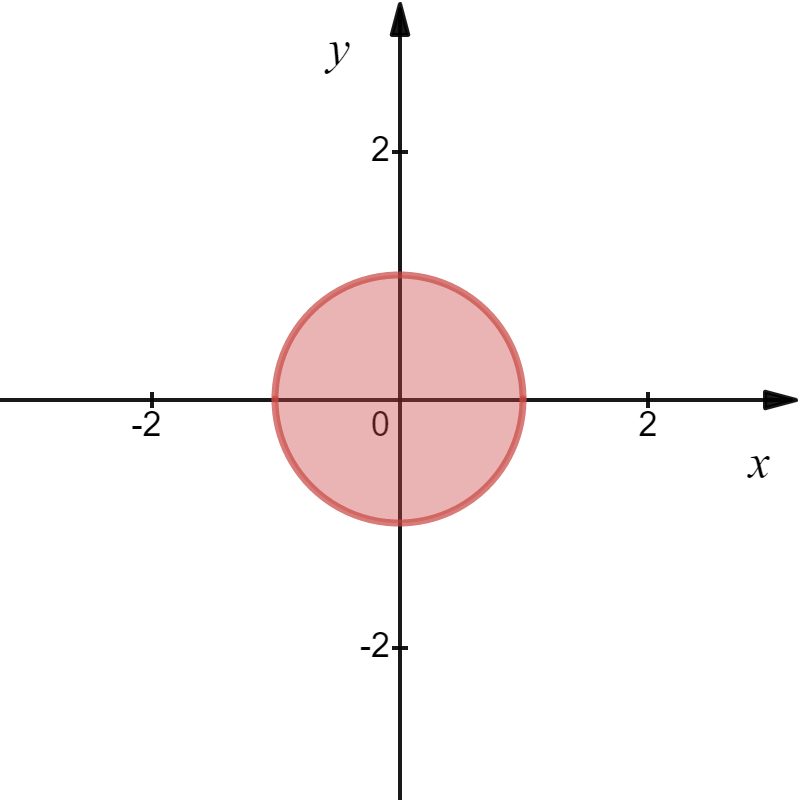
\includegraphics[width=.6\textwidth]{figures/disk.png}
        \caption{Shaded region is the unit disk described by $x^2+y^2\leq 1$.}
    \end{figure}
    Now, if we want just the upper half of this disk, we must require $y\geq 0$, as we can see in the next figure.
    \begin{figure}[H]
        \centering
        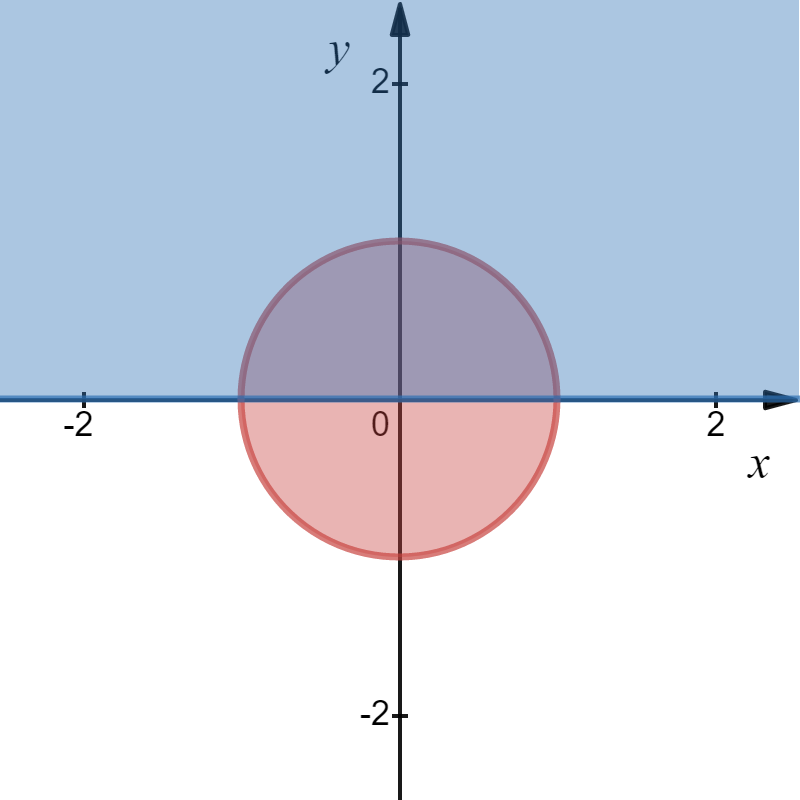
\includegraphics[width=.6\textwidth]{figures/disk_2.png}
        \caption{Red shade region is the unit disk described by $x^2+y^2\leq 1$ and the added constraint $y\geq 0$ is given in blue.}
    \end{figure}
    The overlap of the two colored regions gives us our domain of interest. The last requirement is that we also choose $z=0$. Thus, our parameterization is summarized as
    \begin{align*}
    x^2+y^2 &\leq 1 \\
    y &\geq 0\\
    z &= 0.
    \end{align*}
    Since this is a flat surface in the plane, the normal direction is the $\zhat$ direction. Hence, the surface normal can be chosen to be $\unitvec = \zhat$.
    
    \item We can follow our intuition from the previous part a bit. The surface of the unit sphere is the set of all points in $\R^3$ a distance of 1 away from the origin. The distance from the origin to a point $(x,y,z)$ is $\sqrt{x^2+y^2+z^2}$ again by the Pythagorean theorem. Hence, we have the implicit description
    \[
    \sqrt{x^2+y^2+z^2}=1,
    \]
    for which we could equivalently write
    \[
    x^2+y^2+z^2 =1.
    \]
    One can see previous homeworks for plots of this implicit surface.

    The normal to an implicit surface is $f(x,y,z)=0$ is
    \[
    \unitvec = \frac{\grad f}{|\grad f|},
    \]
    and in our case we have the function
    \[
    f(x,y,z) = x^2+y^2+z^2 -1 = 0.
    \]
    Then, 
    \[
    \grad f = \begin{pmatrix} 2x \\ 2y \\ 2z \end{pmatrix}
    \]
    for which we have
    \[
    |\grad f| = 2\sqrt{x^2+y^2+z^2}.
    \]
    Thus,
    \[
    \unitvec= \frac{x}{\sqrt{x^2+y^2+z^2}} \xhat  + \frac{y}{\sqrt{x^2+y^2+z^2}} \yhat  + \frac{z}{\sqrt{x^2+y^2+z^2}} \zhat.
    \]
\end{enumerate}
\end{solution}

\newpage
\begin{problem}
Consider the following vector field
\[
\vecfieldE(x,y,z) = \begin{pmatrix} \frac{x}{(x^2+y^2+z^2)^{3/2}} \\ \frac{y}{(x^2+y^2+z^2)^{3/2}} \\ \frac{z}{(x^2+y^2+z^2)^{3/2}} \end{pmatrix},
\]
which models the electric field of a proton (in units of of charge $q=1$) placed at the origin.
\begin{enumerate}[(a)]
	\item Show that $\vecfieldE(x,y,z) = - \grad \phi(x,y,z)$ where $\phi(x,y,z) = \frac{1}{\sqrt{x^2+y^2+z^2}}$.  We refer to $\phi(x,y,z)$ as the electrostatic potential (or voltage).
	\item Let $\Omega$ be a box with side lengths two centered at the origin.  Compute the total flux of $\vecfieldE$ through the surface of the box $\Sigma$. That is,
	\[
	\int_\Sigma \vecfieldE \cdot \unitvec d\Sigma.
	\]
	\item Using the provided argument, one can compute
	\[
	\int_\Omega \grad \cdot \vecfieldE d\Omega.
	\]
	\begin{itemize}
		\item Compute $\grad \cdot \vecfieldE$ and note that this is zero everywhere except at $(x,y,z)=(0,0,0)$.
		\item Note that the two integrals in this problem are equal. This is known as the \emph{divergence theorem} and it is a special case of a more general theorem called \emph{Stokes' theorem} which generalizes the fundamental theorem of calculus. Is it true that $\grad \cdot \vecfieldE = 0$ everywhere?
	\end{itemize}
	\item Does the total flux depend on the size or shape of the box?
\end{enumerate}
\end{problem}~
\begin{solution}
    \begin{enumerate}[(a)]
        \item   We compute $-\grad \phi$,
        \begin{align*}
            -\grad \phi &= \begin{pmatrix} -\frac{\partial V}{\partial x} \\ -\frac{\partial V}{\partial y} \\ -\frac{\partial V}{\partial z} \end{pmatrix}\\
            &= \begin{pmatrix} \frac{x}{(x^2+y^2+z^2)^{3/2}} \\ \frac{y}{(x^2+y^2+z^2)^{3/2}} \\ \frac{z}{(x^2+y^2+z^2)^{3/2}} \end{pmatrix}\\
            &= \vecfieldE.
        \end{align*}
        \item This portion requires computing six different (however, symmetric) integrals.  One can reduce the argument down to a single integral via a bit of physical/mathematical reasoning. Note that the field $\vecfieldE$ is radially symmetric in that the field points radially outward from the origin and the strength falls off as we move away from the origin.  Fundamentally, this means that each face of the cube receives the same amount of flux through it. Another way to see this symmetry is if one exchanges $x$ for $y$, $x$ for $z$, 
or $y$ for $z$, the function $\phi$ remains unchanged and so must $\vecfieldE$.
        
        Picture the situation as follows. We have the cube surface broken up into $6$ faces. We will label these faces as $\Sigma_1$, $\Sigma_2,\dots,\Sigma_6$.  
        \begin{figure}[H]
        	\centering
        	\def\svgwidth{0.75\columnwidth}
        	\input{figures/cube_coordinate_axes.pdf_tex}
        \end{figure}
        One can take $\Sigma_4$, $\Sigma_5$, and $\Sigma_6$ to be the faces opposite to $\Sigma_1$, $\Sigma_2$ and $\Sigma_3$ respectively.  Each face then has a unique outward normal vector which we can denote by $\unitvec_{\Sigma_j}$ for the face $\Sigma_j$.
        \begin{figure}[H]
        	\centering
        	\def\svgwidth{0.75\columnwidth}
        	\input{figures/cube_normal_vectors.pdf_tex}
        \end{figure}
        Thus, our integral over the cubic surface $\Sigma$ is given by
        \[
        \iint_{\Sigma} \vecfieldE \cdot \unitevec d\Sigma = \sum_{j=1}^6 \iint_{\Sigma_j} \vecfieldE \cdot \unitvec_{\Sigma_j}d\Sigma_j.
        \]
        By the symmetry argument before, we can simplify this further as
        \[
        \iint_\Sigma \vecfieldE \cdot \unitvec d\Sigma = 6 \iint_{\Sigma_1} \vecfieldE \cdot \unitvec_{\Sigma_1}d\Sigma_1.
        \]
        Now, we can evaluate this integral
        \begin{align*}
            6\iint_{\Sigma_1} \vecfieldE \cdot \unitvec_{\Sigma_1}d\Sigma_1 &= \int_{-1}^1 \int_{-1}^1 \vecfieldE(x,y,1) \cdot \zhat dxdy\\&= 6\int_{-1}^1 \int_{-1}^1 \frac{1}{(x^2+y^2+1)^{3/2}}dxdy\\
                &= 6\frac{2\pi }{3}\\
                &= 4\pi.
        \end{align*}
    Note that this integral was computed by inputting the following statement into WolframAlpha:
    \begin{verbatim}
    integrate[integrate[1/(x^2+y^2+1)^(3/2),{x,-1,1}],{y,-1,1}]
    \end{verbatim}

    \item We have already computed $\grad \cdot \vecfieldE$ and noted this in an earlier homework problem.  It's now very physically reasonable to suspect that we have the following identity
    \[
    \int_\Omega \grad \cdot \vecfieldE d\Omega = \int_\Sigma \vecfieldE \cdot \unitvec d\Sigma,
    \]
    since the amount of ``source behavior" in the region $\Omega$ should directly correspond to the flux that will pass through the boundary.  To picture this literally, if we pump in water at $(0,0,0)$, we know how much water we pumped in by seeing how much flows through any surface surrounding the origin. Anyhow, this identity is given in the problem statement so we can take it as truth.
    
    Thus, our argument is that
    \[
    \int_\Omega \grad \cdot \vecfieldE d\Omega = 4\pi.
    \]
    Now, $\grad\cdot \vecfieldE$ is zero aside from at the point $(x,y,z)=(0,0,0)$ where we have a discontinuity in the field. But, if this above integral is nonzero, it must be that $\grad \cdot \vecfieldE \neq 0$ everywhere! 

    Furthermore, we can relate this to the Maxwell equation for the electric field $\vecfieldE$ due to a charge distribution $\rho(x,y,z)$, i.e.,
    \[
    \grad \cdot \vecfieldE = \rho/\epsilon_0.
    \]
    It seems as if all of the charge is concentrated solely at the origin. This is an odd phenomenon we will discuss in more detail later in this course.

    \item From the previous part, we can note that the divergence of $\vecfieldE$ is zero everywhere aside from the origin.  Hence, the only possible source of flux comes from the origin and our previous argument discussed the symmetry of this field.  So, no, the flux does not depend on the shape or size of the box so long as we integrate about a surface that encloses the origin.
    \end{enumerate}
\end{solution}

\end{document}